% Created 2019-02-21 ju. 23:14
% Intended LaTeX compiler: pdflatex
\documentclass[xcolor={usenames,svgnames,dvipsnames}]{beamer}
\usepackage[utf8]{inputenc}
\usepackage[T1]{fontenc}
\usepackage{graphicx}
\usepackage{grffile}
\usepackage{longtable}
\usepackage{wrapfig}
\usepackage{rotating}
\usepackage[normalem]{ulem}
\usepackage{amsmath}
\usepackage{textcomp}
\usepackage{amssymb}
\usepackage{capt-of}
\usepackage{hyperref}
\usepackage{color}
\usepackage{listings}
\usepackage[spanish]{babel}
\usecolortheme{rose}
\setbeamercolor{alerted text}{fg=Blue}
\setbeamerfont{alerted text}{series=\bfseries}
\setbeamerfont{block title}{series=\bfseries}
\setbeamercolor{block title}{bg=structure.fg!20!bg!50!bg}
\setbeamercolor{block body}{use=block title,bg=block title.bg}
\setbeamertemplate{navigation symbols}{}
\AtBeginSection[]{\begin{frame}[plain]\tableofcontents[currentsection,sectionstyle=show/shaded, subsectionstyle=show/hide]\end{frame}}
\AtBeginSubsection[]{\begin{frame}[plain]\tableofcontents[currentsubsection,sectionstyle=show/shaded,subsectionstyle=show/shaded/hide]\end{frame}}
\lstset{keywordstyle=\color{blue}, commentstyle=\color{gray!90}, basicstyle=\ttfamily\small, columns=fullflexible, breaklines=true,linewidth=\textwidth, backgroundcolor=\color{gray!23}, basewidth={0.5em,0.4em}, literate={¡}{{\textexclamdown}}1 {á}{{\'a}}1 {ñ}{{\~n}}1 {é}{{\'e}}1 {ó}{{\'o}}1 {í}{{\'i}}1 {ú}{{\'u}}1 {º}{{\textordmasculine}}1, showstringspaces=false}
\usepackage{mathpazo}
\hypersetup{colorlinks=true, linkcolor=Blue, urlcolor=Blue}
\usepackage{fancyvrb}
\DefineVerbatimEnvironment{verbatim}{Verbatim}{fontsize=\tiny, formatcom = {\color{black!70}}}
\beamertemplatenavigationsymbolsempty
\setbeamertemplate{footline}[frame number]
\usetheme{Goettingen}
\usefonttheme{serif}
\author{Oscar Perpiñán Lamigueiro}
\date{}
\title{Introducción al control de versiones y trabajo colaborativo con GitHub}
\hypersetup{
 pdfauthor={Oscar Perpiñán Lamigueiro},
 pdftitle={Introducción al control de versiones y trabajo colaborativo con GitHub},
 pdfkeywords={},
 pdfsubject={},
 pdfcreator={Emacs 26.1 (Org mode 9.1.14)}, 
 pdflang={Spanish}}
\begin{document}

\maketitle

\section{Conceptos básicos}
\label{sec:orgf9a9788}
\subsection{¿Qué es el control de versiones?}
\label{sec:org75a3f24}

\begin{frame}[plain,label={sec:orgce288af}]{}
\begin{center}

\includegraphics[width=0.9\paperwidth]{figs/phdcomic_finaldoc_1.png}
\end{center}

\url{http://phdcomics.com/comics/archive.php?comicid=1531}
\end{frame}

\begin{frame}[plain,label={sec:org311f4e6}]{}
\begin{center}

\includegraphics[width=0.9\paperwidth]{figs/phdcomic_finaldoc_2.png}
\end{center}

\url{http://phdcomics.com/comics/archive.php?comicid=1531}
\end{frame}

\begin{frame}[plain,label={sec:org42a1ff1}]{}
\begin{center}
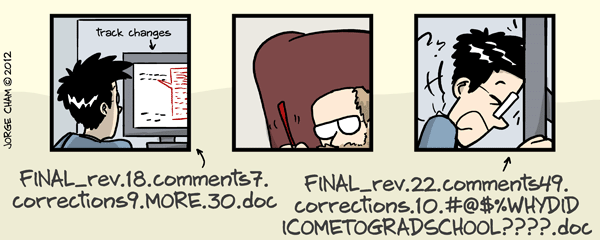
\includegraphics[width=0.9\paperwidth]{figs/phdcomic_finaldoc_3.png}
\end{center}

\url{http://phdcomics.com/comics/archive.php?comicid=1531}
\end{frame}

\begin{frame}[label={sec:orgabc4671}]{¿Qué es el control de versiones y por qué debería importarte?}
\begin{quote}
El control de versiones es un sistema que \alert{registra los cambios}
realizados sobre un archivo o conjunto de archivos a lo largo del
tiempo, de modo que se puedan \alert{recuperar} versiones específicas más
adelante.\footnote{\url{https://git-scm.com/book/es/v1/Empezando-Acerca-del-control-de-versiones}}
\end{quote}
\end{frame}

\begin{frame}[label={sec:orgac40155}]{¿Qué es el control de versiones y por qué debería importarte?}
\begin{quote}
El control de versiones es el cuaderno de laboratorio en el
mundo digital. 

Es lo que los profesionales usan para realizar un
\alert{seguimiento} de lo que han hecho y para \alert{colaborar} con otras
personas. 

\alert{No sirve sólo para software}: libros, documentos, pequeños
conjuntos de datos y cualquier cosa que cambie con el tiempo o que
deba compartirse puede y debe almacenarse en un sistema de control de
versiones.\footnote{\url{https://swcarpentry.github.io/git-novice/}}
\end{quote}
\end{frame}

\begin{frame}[label={sec:org92452b6}]{Viajar en el tiempo}
\begin{itemize}
\item Nada que haya sido sometido a un control de versiones se pierde jamás (\emph{salvo que realmente quieras eliminarlo\ldots{}})
\item \alert{Todas} las versiones antiguas de un fichero se almacenan: un fichero se puede revertir a un estado anterior sin límites.
\end{itemize}
\end{frame}
\begin{frame}[label={sec:orgc6eebeb}]{¿Qué? ¿Cuándo? ¿Quién?}
Un sistema de control de versiones registra:
\begin{itemize}
\item El detalle de los cambios realizados.
\item La fecha y hora en la que fueron realizados.
\item La persona que los realizó.
\end{itemize}
\end{frame}

\begin{frame}[label={sec:org0eef87d}]{Trabajo Colaborativo}
\begin{itemize}
\item Cuando un equipo de personas trabaja conjuntamente en un proyecto, es posible que se produzcan cambios incompatibles en un mismo fichero.
\item El sistema de control de versiones \alert{impide} cambios simultáneos en un fichero. A cambio, permite la \alert{resolución de conflictos} y los documenta.
\end{itemize}
\end{frame}

\subsection{¿Qué son Git y GitHub?}
\label{sec:orgc602319}

\begin{frame}[fragile,label={sec:org152d32c}]{Git es un Sistema de Control de Versiones}
 Git es una herramienta software (accesible mediante línea de comandos con \texttt{git}) que implementa un Sistema de Control de Versiones.

\begin{center}
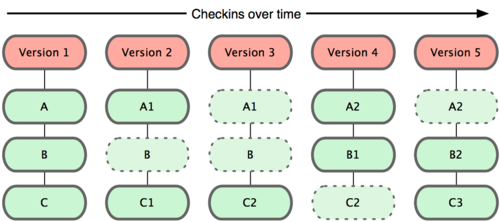
\includegraphics[width=.9\linewidth]{figs/git_model.png}
\end{center}
\end{frame}

\begin{frame}[label={sec:org8e66a76}]{Git es un Sistema de Control de Versiones}
Cada vez que se ejecuta un cambio en una estructura de ficheros controlada con Git, realiza una \guillemotleft{}foto\guillemotright{} del estado de los archivos en ese momento, y guarda una referencia a esa instantánea. 
\begin{center}
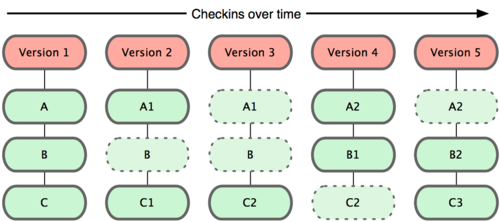
\includegraphics[width=.9\linewidth]{figs/git_model.png}
\end{center}
\end{frame}

\begin{frame}[label={sec:orgc3c776c}]{Git es un Sistema de Control de Versiones}
Por eficiencia, Git no almacena los archivos sin modificaciones sino un enlace al archivo anterior idéntico que ya está almacenado

\begin{center}
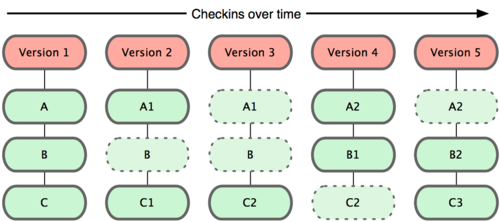
\includegraphics[width=.9\linewidth]{figs/git_model.png}
\end{center}
\end{frame}

\begin{frame}[label={sec:orgf7bd5e2}]{Los estados de Git}
\begin{itemize}
\item El desarrollador incorpora uno o varios ficheros al control de versiones. (\emph{tracked})
\item Realiza modificaciones en los ficheros (\emph{modified}).
\item Incorpora esos ficheros modificados al área de preparación (\emph{staged}).
\item Finalmente, confirma todos los cambios del área de preparación: se realiza la instantánea de los ficheros. (\emph{committed})
\end{itemize}
\begin{center}
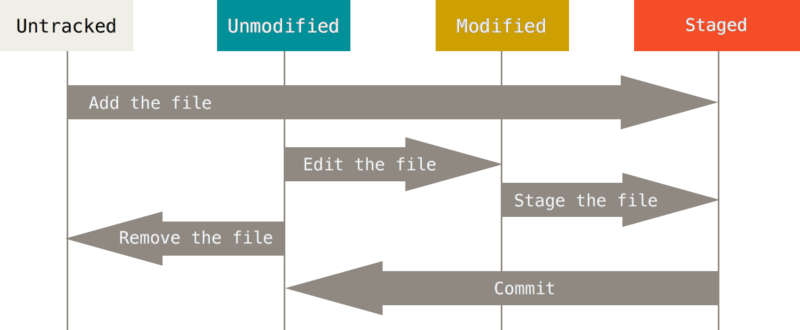
\includegraphics[height=0.4\textheight]{figs/git_estados.png}
\end{center}
\end{frame}

\begin{frame}[fragile,label={sec:org2e18ac9}]{¿Qué es GitHub?}
 \begin{itemize}
\item GitHub es la plataforma de alojamiento de código más importante a nivel mundial.
\item Emplea el sistema de control de versiones \texttt{git}
\item Ofrece una amplia variedad de funcionalidades
\begin{itemize}
\item Alojamiento de código
\item Revisión de código
\item Trabajo colaborativo
\item Publicación de páginas web
\end{itemize}
\end{itemize}
\end{frame}

\section{Uso de \texttt{git} y \texttt{GitHub}}
\label{sec:orgda4d373}

\subsection{Primeros Pasos}
\label{sec:org9b0bbdf}
\begin{frame}[label={sec:org0ded2ac}]{Creación de una cuenta en GitHub}
\url{https://github.com/join}

\begin{center}
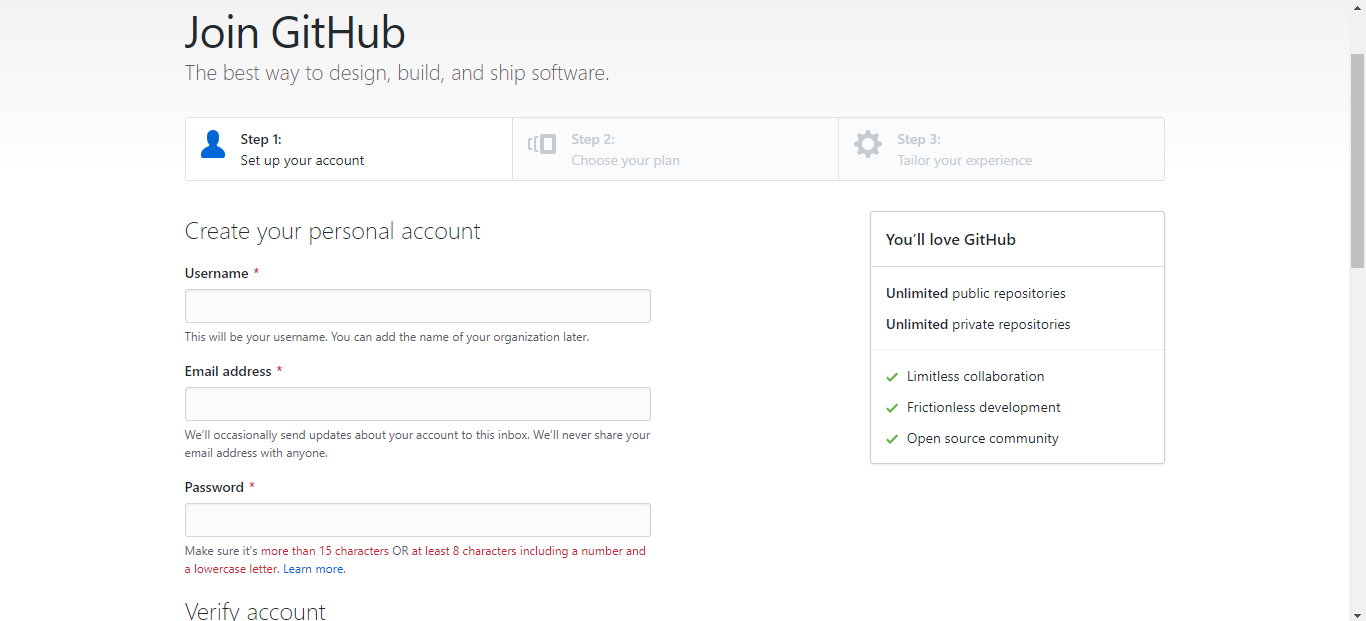
\includegraphics[width=.9\linewidth]{figs/GitHub_Join.png}
\end{center}

Más información en \href{https://help.github.com/articles/signing-up-for-a-new-github-account/}{New GitHub account}
\end{frame}

\begin{frame}[label={sec:org553277d}]{Instalación de GitHub Desktop}
\url{https://desktop.github.com/}

\begin{center}

\includegraphics[width=.9\linewidth]{figs/GitHub_Desktop.png}
\end{center}
\end{frame}

\begin{frame}[label={sec:org6f19e8b}]{Conectamos Git, GitHub y GitHub Desktop}
\begin{itemize}
\item Una vez instalado comienza el proceso de autenticación, usando las credenciales del paso anterior\footnote{Más información en \href{https://help.github.com/desktop/guides/getting-started-with-github-desktop/authenticating-to-github/}{Authenticating to GitHub}.}.
\end{itemize}

\begin{center}
\boxed{File > Options > Accounts > Sign\ In}
\end{center}


\begin{itemize}
\item A continuación, conectamos la información de usuario con Git\footnote{Más información en \href{https://help.github.com/desktop/guides/getting-started-with-github-desktop/configuring-git-for-github-desktop/}{Configuring Git}.}.
\end{itemize}

\begin{center}
\boxed{File > Options > Git}
\end{center}
\end{frame}

\begin{frame}[fragile,label={sec:orgad684ca}]{Remoto y Local}
 \begin{itemize}
\item \alert{Github.com} aloja los \alert{repositorios remotos} (nube).
\item En tu ordenador trabajas con una \alert{copia local} del repositorio. Otros desarrolladores tendrán sus propias copias locales.
\item La(s) copia(s) local(es) y el repositorio remoto deben estar \alert{sincronizados} mediante diferentes comandos de \texttt{git}.
\end{itemize}
\end{frame}

\begin{frame}[label={sec:org95be6e8}]{Nuevo repositorio \emph{remoto} desde github.com}
\url{https://github.com/new}

\begin{center}
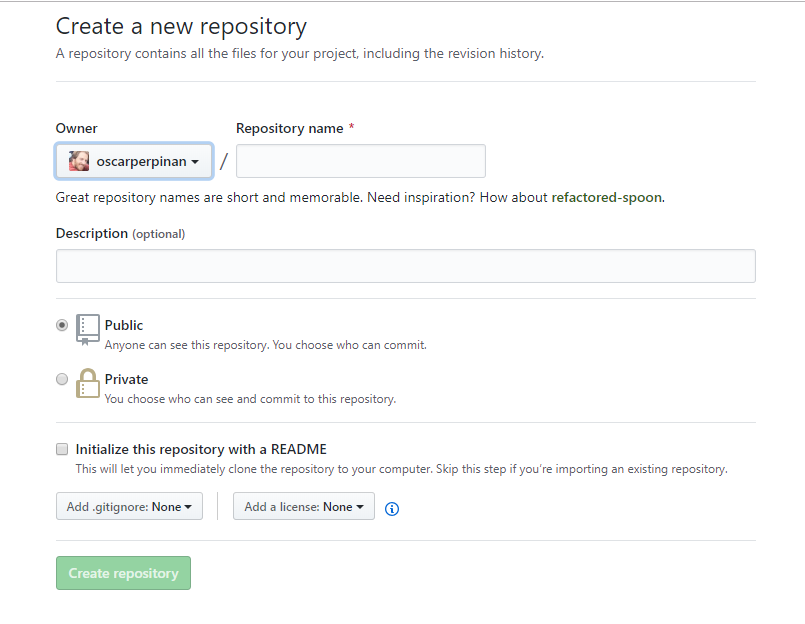
\includegraphics[width=.9\linewidth]{figs/GitHub_New_Repository.png}
\end{center}
\end{frame}

\begin{frame}[label={sec:org5bb96d9}]{Nuevo repositorio \emph{local} desde GitHub Desktop}
\begin{center}
\boxed{File > New\ Repository}
\end{center}

\begin{center}
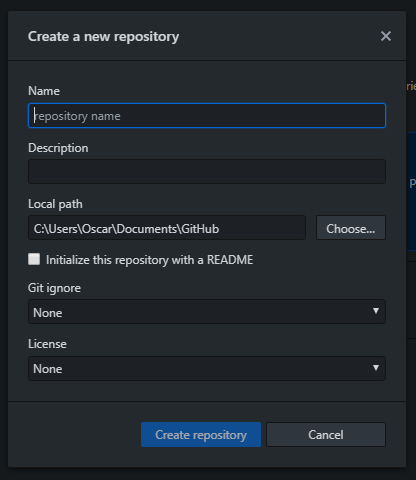
\includegraphics[height=0.7\textheight]{figs/Desktop_NewRepository.png}
\end{center}
\end{frame}

\begin{frame}[fragile,label={sec:org28ec52b}]{Decisiones al crear un repositorio}
 \begin{itemize}
\item Elige un \alert{\texttt{.gitignore}} adecuado al proyecto: Veáse \url{https://github.com/github/gitignore}.
\item No olvides inicializar y cumplimentar el \alert{\texttt{README.md}}. Para el formato veáse \href{https://help.github.com/articles/basic-writing-and-formatting-syntax/}{Formatting syntax}.
\item Elige una \alert{licencia} adecuada a tu proyecto y a tus intereses actuales y futuros. Veáse \url{https://choosealicense.com}.
\end{itemize}
\end{frame}

\begin{frame}[label={sec:org0a5f60c}]{Clonar un repositorio remoto}
Si hemos creado el repositorio desde github.com (\emph{repositorio remoto}), hay que clonarlo para poder trabajar con él (\emph{copia local}).

\begin{center}
\boxed{File > Clone\ Repository}
\end{center}

\begin{center}
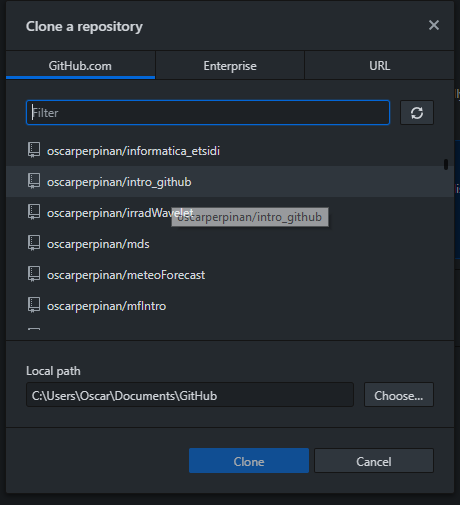
\includegraphics[height=0.65\textheight]{figs/Desktop_CloneRepository.png}
\end{center}
\end{frame}

\begin{frame}[label={sec:org2fdbae6}]{Publicar un repositorio local}
Si hemos creado el repositorio desde GitHub Desktop (\emph{repositorio local}), hay que publicarlo en github.com (\emph{repositorio remoto})

\begin{center}
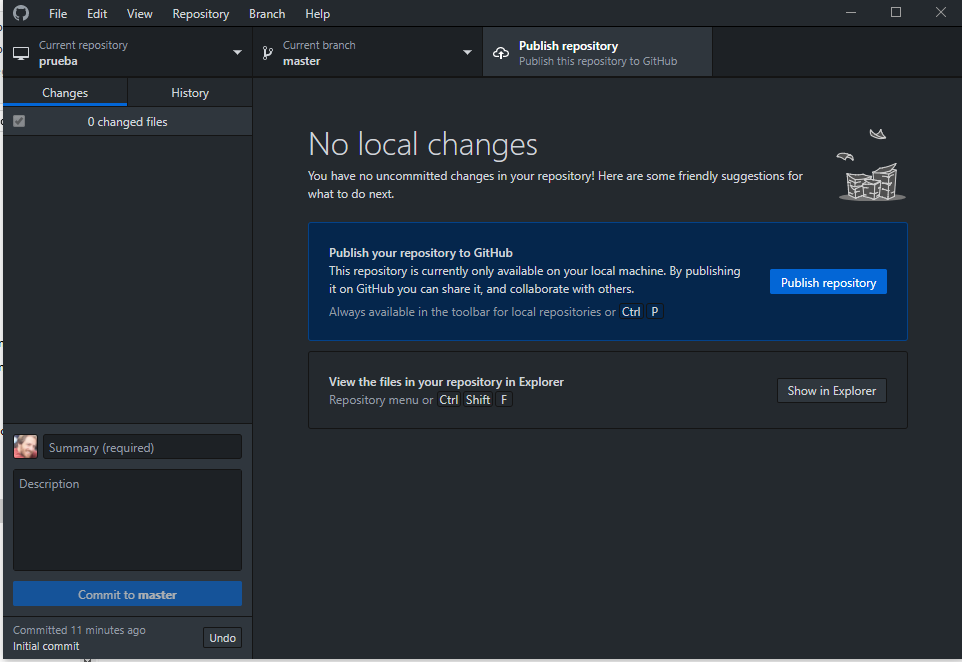
\includegraphics[width=.9\linewidth]{figs/Desktop_PublishRepository.png}
\end{center}
\end{frame}


\subsection{Flujo de Trabajo}
\label{sec:org61b9326}

\begin{frame}[fragile,label={sec:org9e7e0d1}]{Cambios en la copia local}
 \begin{enumerate}
\item Modifica los ficheros de la copia local.
\item Añade los cambios realizados a la siguiente \guillemotleft{}instantánea\guillemotright{} del repositorio (\texttt{git add}) \begin{center}
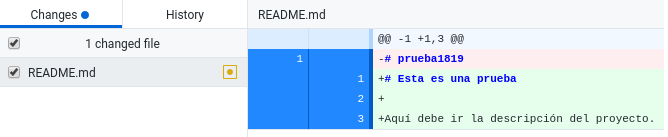
\includegraphics[width=.9\linewidth]{figs/git_add.png}
\end{center}
\item Confirma los cambios, escribiendo un resumen de lo realizado (\texttt{git commit})
\begin{center}
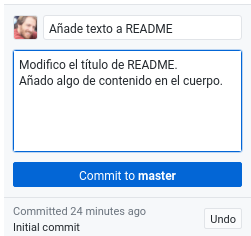
\includegraphics[height=0.3\textheight]{figs/git_commit.png}
\end{center}
\end{enumerate}
\end{frame}
\begin{frame}[fragile,label={sec:org51ac2a6}]{Como escribir un buen mensaje de \texttt{commit}}
 \begin{itemize}
\item \emph{Commit early and often}: cada \texttt{commit} debe incluir cambios pequeños y coherentes.

\item Escribir un mensaje de calidad al ejecutar cambios facilita tanto el trabajo personal como la colaboración en equipo con Git.\footnote{\url{https://chris.beams.io/posts/git-commit/}}
\end{itemize}
\begin{block}{Recomendaciones}
\begin{itemize}
\item El \alert{título} debe ser \alert{conciso} (50 caracteres) y escrito en imperativo (\emph{Do something\ldots{}})
\item El \alert{cuerpo} debe explicar \alert{el qué y el por qué del cambio}, no el cómo, comparando con el comportamiento anterior al cambio.
\item Se pueden incluir referencias a \emph{issues} (ver a continuación) con \#XX siendo XX el número de la \emph{issue}.
\end{itemize}
\end{block}
\end{frame}
\begin{frame}[fragile,label={sec:org10f4241}]{Histórico de cambios}
 Los cambios confirmados con \texttt{commit} se anotan en la historia (\texttt{git log})

\begin{center}
\boxed{View > History}
\end{center}

\begin{center}
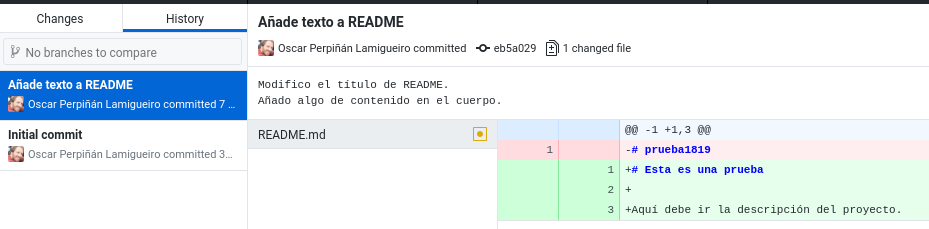
\includegraphics[width=.9\linewidth]{figs/git_history.png}
\end{center}
\end{frame}


\begin{frame}[fragile,label={sec:orge6a0857}]{Publicar cambios al repositorio remoto}
 \begin{itemize}
\item Para sincronizar  los cambios realizados \alert{desde la copia local hasta el repositorio remoto} hay que publicar mediante \texttt{git push}.
\end{itemize}

\begin{center}
\boxed{Repository > Push}
\end{center}

\begin{itemize}
\item A partir de este punto, la copia local y el repositorio remoto están sincronizados.
\end{itemize}

\begin{block}{Importante}
En el caso de repositorios compartidos, antes de un \texttt{git push} es imprescindible actualizar la copia local incorporando los cambios del repositorio con \texttt{git pull}.
\end{block}
\end{frame}
\begin{frame}[fragile,label={sec:org17ed654}]{Recibir cambios de un repositorio remoto}
 Para obtener en la copia local los cambios recientes que existan en el repositorio hay que emplear \texttt{git pull}, que es la combinación de la secuencia:
\begin{enumerate}
\item \texttt{git fetch}, para obtener los cambios recientes del repositorio remoto.
\item \texttt{git merge}, para combinarlos con la copia local.
\end{enumerate}

\begin{center}
\boxed{Repository > Pull}
\end{center}
\end{frame}
\begin{frame}[label={sec:org6f1c6d3}]{Resumen}
\begin{enumerate}
\item Realiza modificaciones en los ficheros de la copia local.
\item \alert{COMMIT} :: Confirma los cambios con un mensaje informativo.
\item \alert{PULL} :: Incorpora los cambios del repositorio remoto a la copia local.
\item \alert{PUSH} :: Publica los cambios de la copia local al repositorio remoto.
\end{enumerate}
\end{frame}
\section{Trabajo en colaboración}
\label{sec:org4fc8dc4}
\subsection{Ramas}
\label{sec:org35eea5e}

\begin{frame}[fragile,label={sec:orge495c86}]{Rama \texttt{master}}
 \begin{center}
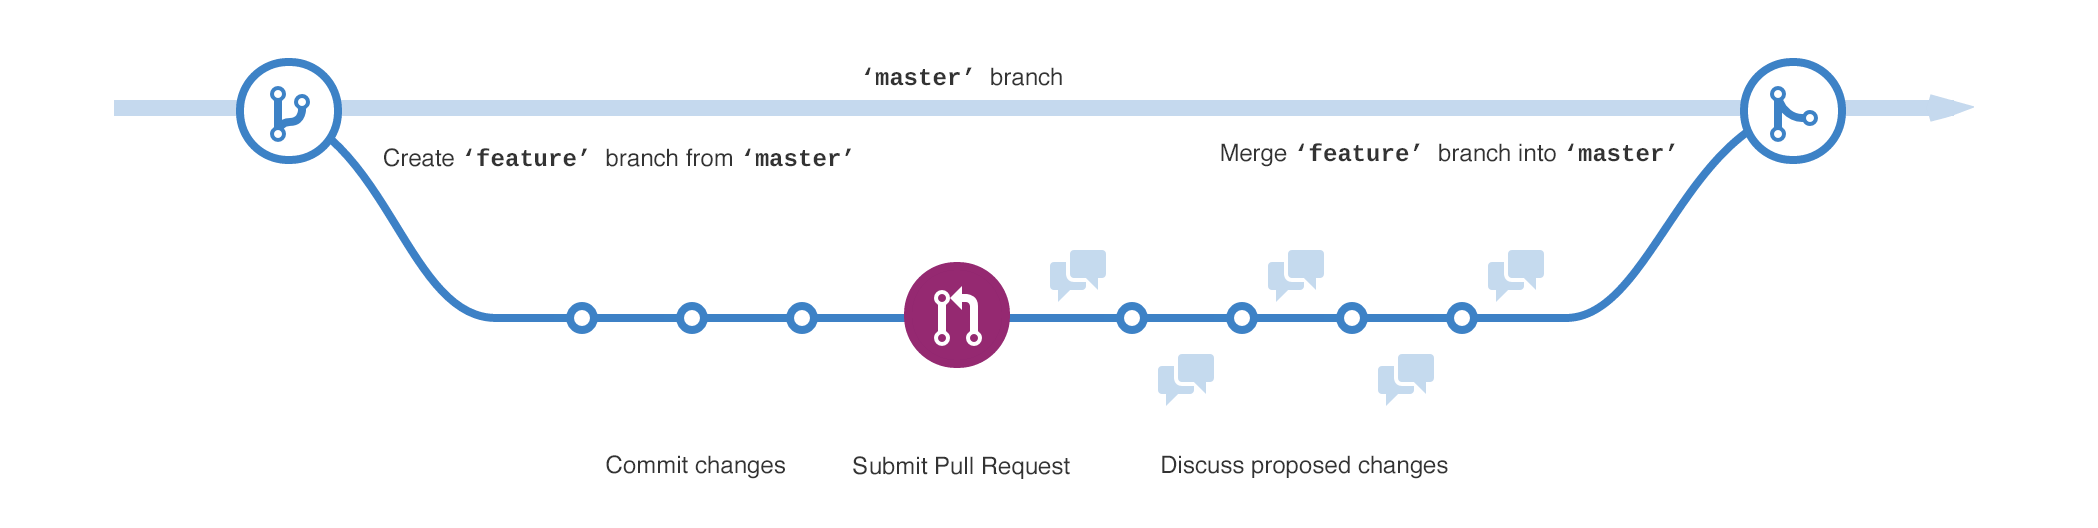
\includegraphics[width=.9\linewidth]{figs/branching.png}
\end{center}

En un repositorio de GitHub existe una rama (\emph{branch}) que se usa por defecto: \alert{master}\footnote{\href{https://guides.github.com/introduction/flow/}{Understanding the GitHub Flow}}.
\end{frame}

\begin{frame}[label={sec:org4af39c2}]{Ramas para facilitar la colaboración}
\begin{center}
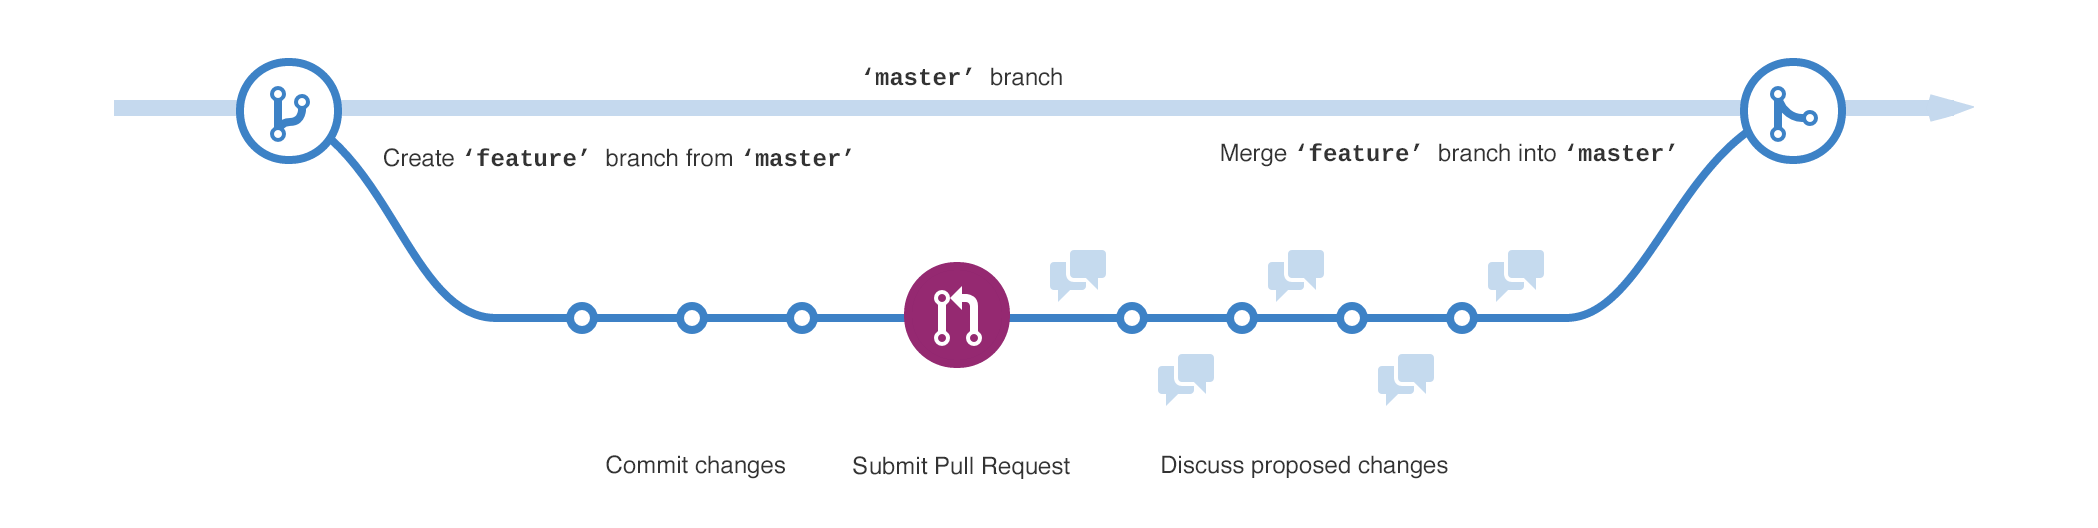
\includegraphics[width=.9\linewidth]{figs/branching.png}
\end{center}

\begin{columns}
\begin{column}{0.6\columnwidth}
Cuando hay varias personas trabajando sobre un mismo repositorio, es necesario crear nuevas ramas para evitar conflictos. 

De esta forma, cada persona implementa \alert{cambios} en una \alert{rama determinada} de forma paralela al resto del equipo.
\end{column}

\begin{column}{0.4\columnwidth}
\begin{center}
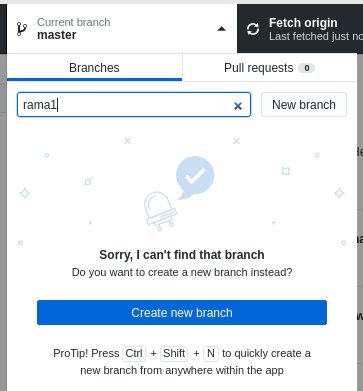
\includegraphics[width=.9\linewidth]{figs/nueva_rama_desktop.png}
\end{center}
\end{column}
\end{columns}
\end{frame}

\begin{frame}[label={sec:orgb152c2e}]{Combinación de código}
\begin{center}
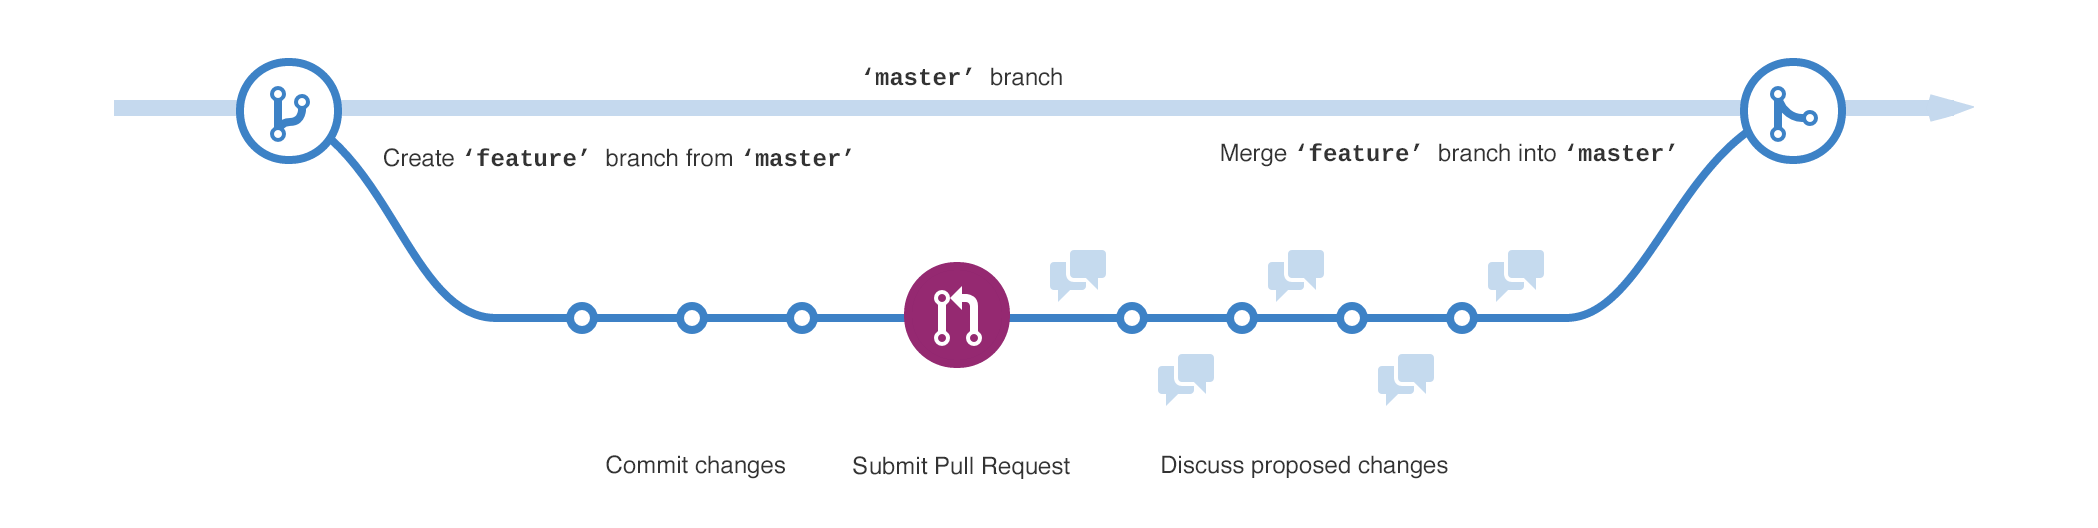
\includegraphics[width=.9\linewidth]{figs/branching.png}
\end{center}

Cuando los cambios están listos y confirmados (\emph{commit} + \emph{push} en la rama específica), se realiza una petición (\emph{pull request}) para combinar estos cambios en la rama \alert{master}.

\begin{columns}
\begin{column}{0.45\columnwidth}
\begin{center}
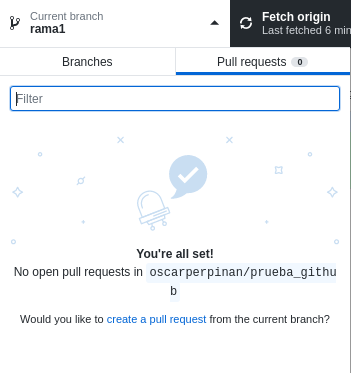
\includegraphics[width=.9\linewidth]{figs/pull_request_desktop.png}
\end{center}
\end{column}

\begin{column}{0.45\columnwidth}
\begin{center}
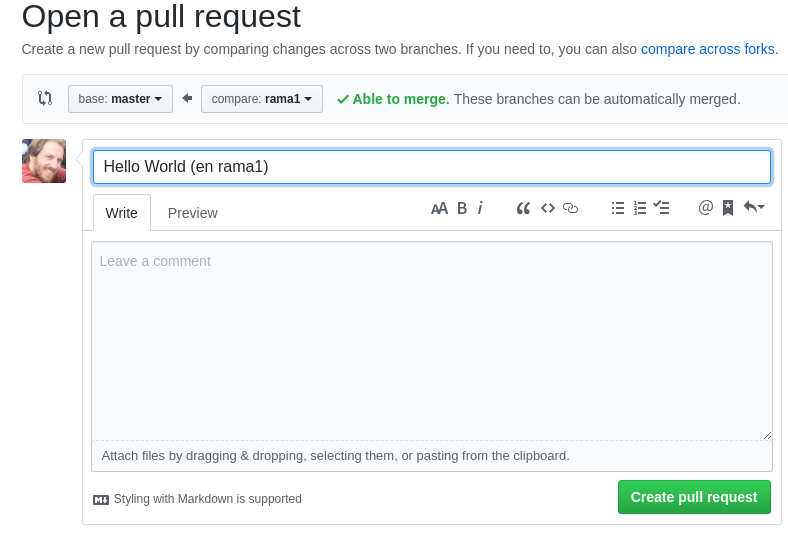
\includegraphics[width=.9\linewidth]{figs/pull_request_web.png}
\end{center}
\end{column}
\end{columns}
\end{frame}

\begin{frame}[label={sec:orgdd4aac3}]{Combinación de código}
\begin{center}
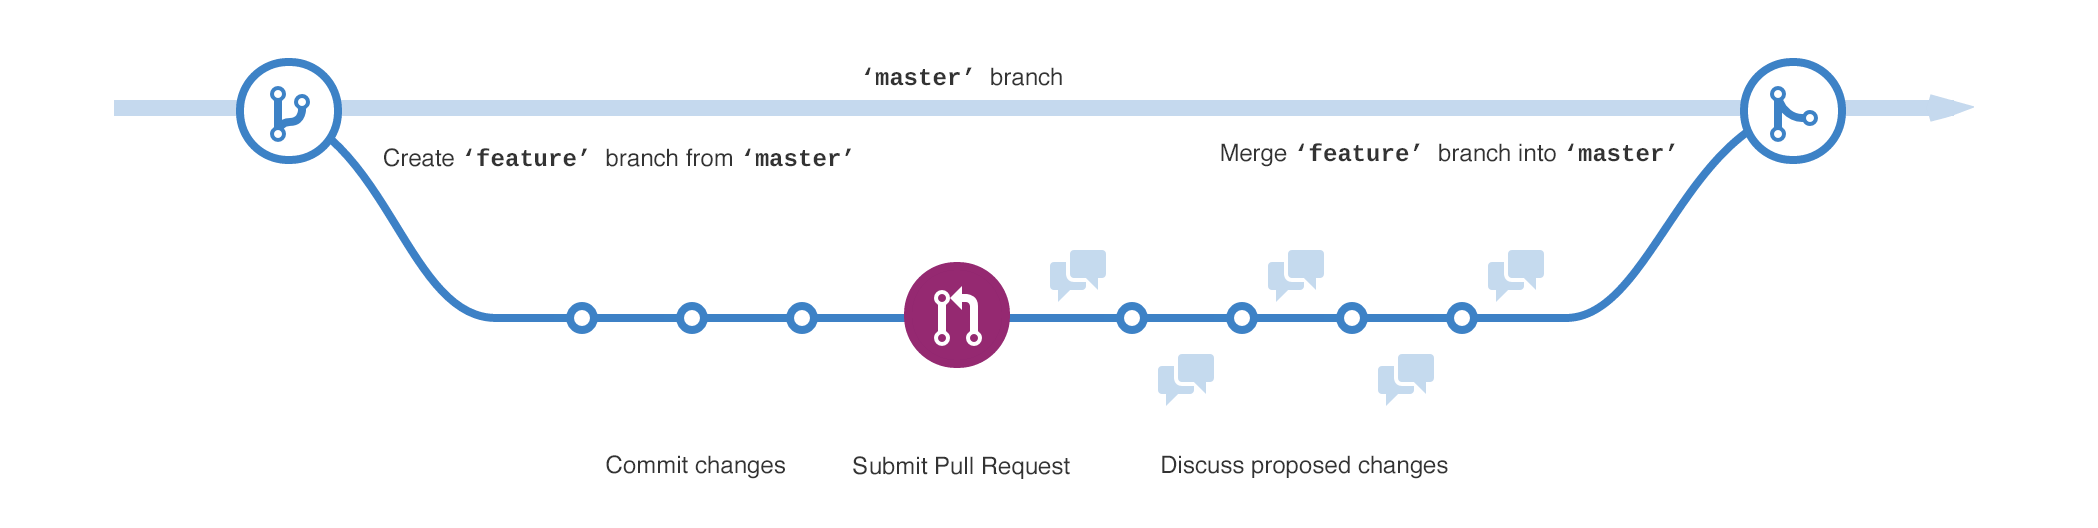
\includegraphics[width=.9\linewidth]{figs/branching.png}
\end{center}


El coordinador del proyecto es el encargado de revisar cada petición y, si todo está correcto, incluir los cambios (\emph{merge}) en la rama \alert{master}. 

\begin{center}
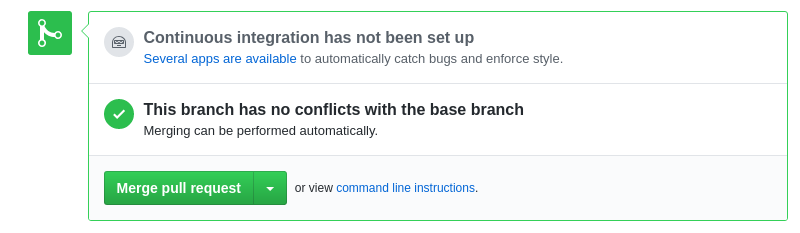
\includegraphics[width=.9\linewidth]{figs/merge_pull_request.png}
\end{center}
\end{frame}

\begin{frame}[label={sec:org323838e}]{Resolución de conflictos}
Si no se pueden combinar los cambios automáticamente se produce un conflicto (por ejemplo, cuando dos usuarios modifican un mismo fichero).

\begin{center}
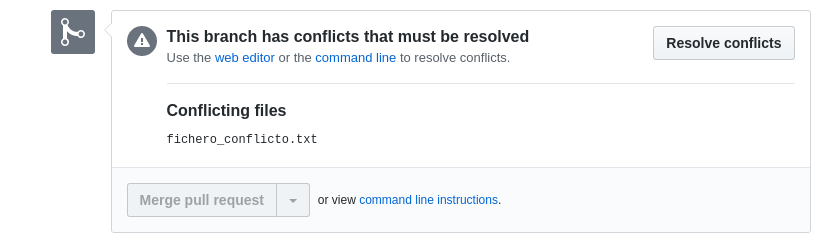
\includegraphics[width=.9\linewidth]{figs/conflict_web.png}
\end{center}

Un conflicto se debe resolver manualmente.
\begin{center}
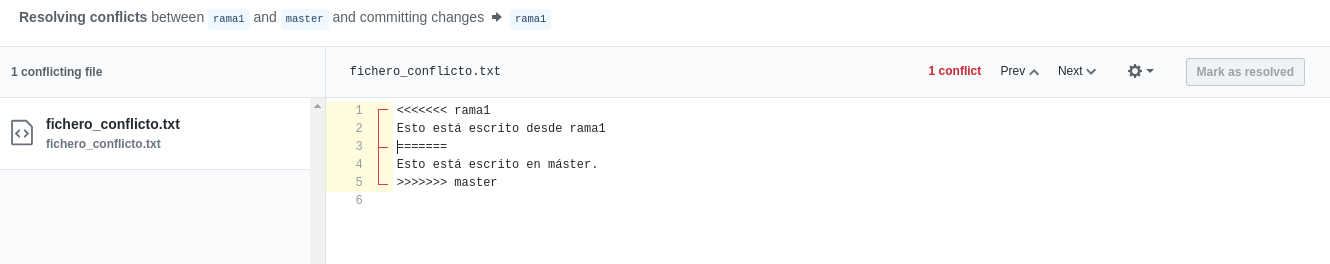
\includegraphics[width=.9\linewidth]{figs/resolve_conflict_web.png}
\end{center}
\end{frame}

\begin{frame}[fragile,label={sec:orga2caa9b}]{Consejos}
 \begin{itemize}
\item \alert{No olvides hacer \emph{pull} antes de iniciar una nueva interacción con el repositorio}.

\item Recuerda las recomendaciones sobre un buen mensaje de \texttt{git commit}.

\item \alert{Organización previa}: las \alert{tareas} asignadas a un rama deben ser \alert{independientes} de las otras ramas para evitar conflictos.

\item Cuando el trabajo en una rama ha concluido, hay que \alert{combinar cambios con master lo antes posible} para reducir la posibilidad de conflicto. Las ramas accesorias utilizadas se pueden eliminar una vez finalizado el proceso.

\item Este proceso se debe repetir tantas veces como sea necesario para realizar cambios de forma colaborativa.
\end{itemize}
\end{frame}

\subsection{Persiguiendo a los bichos}
\label{sec:orge2b8a67}

\begin{frame}[label={sec:org54572c5}]{Issues}
Todos los repositorios de GitHub tienen una sección denominada \guillemotleft{}Issues\guillemotright{}\footnote{\url{https://guides.github.com/features/issues/}} a modo de \emph{bug tracker}.

Pueden usarse para seguimiento de fallos, mejoras, tareas, etc.

\begin{center}
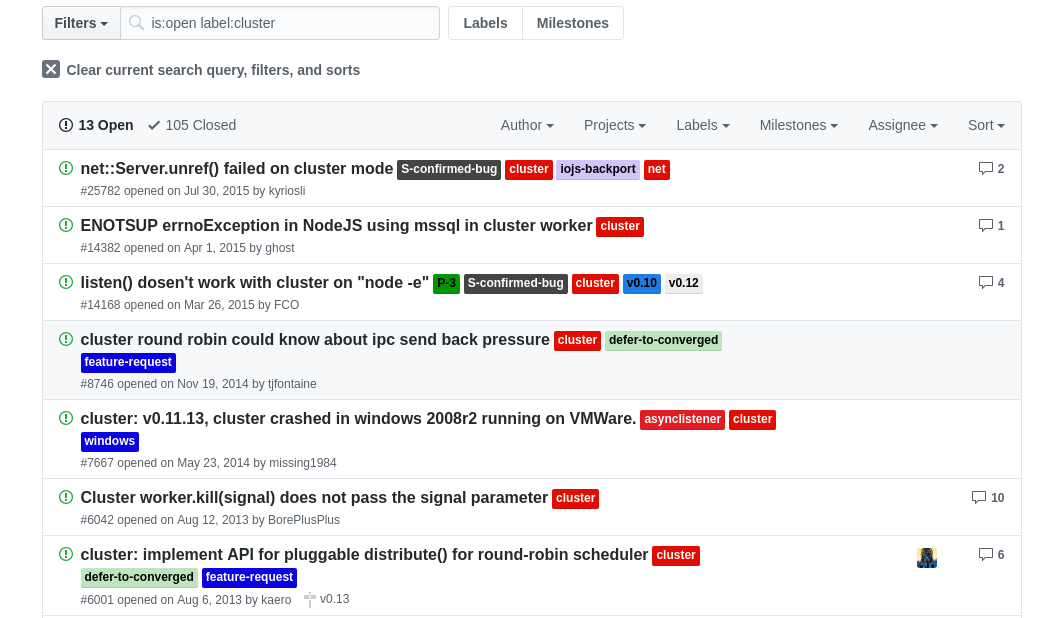
\includegraphics[width=.9\linewidth]{figs/github_issues.png}
\end{center}
\end{frame}

\begin{frame}[label={sec:org6005b67}]{Estructura de una issue}
Una issue es un tablero de discusión en el que pueden participar los responsables del repositorio y cualquier usuario de GitHub.

\alert{Debe} contener un título y una descripción.

\alert{Puede} contener etiquetas, metas, y responsables.

\begin{center}
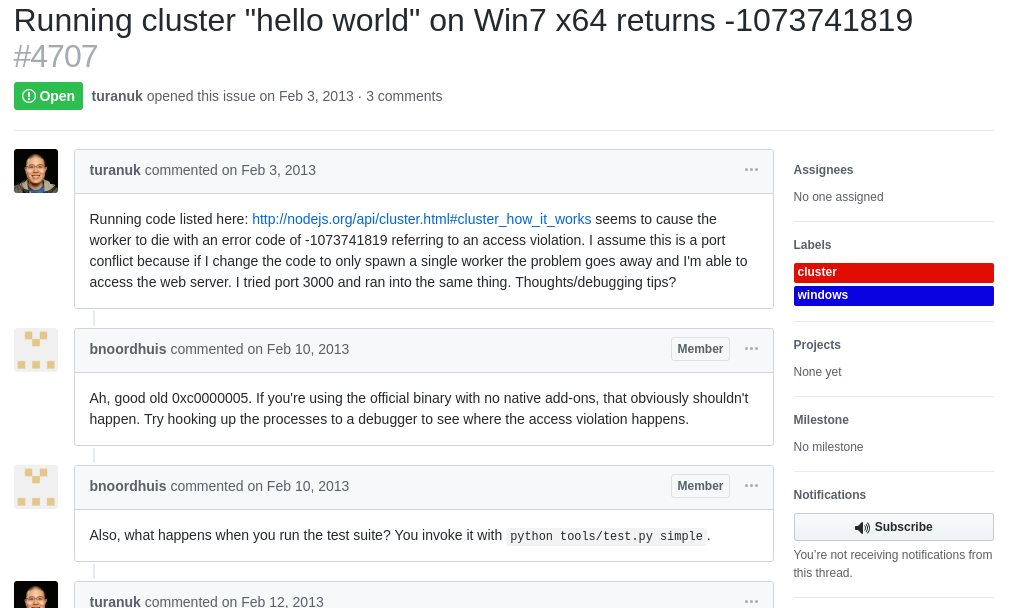
\includegraphics[width=.9\linewidth]{figs/github_issue_example.png}
\end{center}
\end{frame}

\begin{frame}[label={sec:org35d97a9}]{Contenido de una issue}
\begin{itemize}
\item En la descripción de una issue se debe suministrar toda la información posible para el responsable del repositorio, \alert{incluyendo un ejemplo mínimo, completo y verificable}\footnote{\url{https://stackoverflow.com/help/mcve}}.

\item El contenido será formateado como Markdown (incluye un \emph{preview})\footnote{Veáse la guía \href{https://help.github.com/articles/basic-writing-and-formatting-syntax/}{Basic Writing and Formatting syntax}.}.

\item Se pueden incluir referencias al código y a otras issues\footnote{Veáse la guía \href{https://help.github.com/articles/autolinked-references-and-urls/}{Autolinked references and urls}.}.
\end{itemize}
\end{frame}


\subsection{Herramientas gráficas para el análisis de un repositorio}
\label{sec:orgb550a1b}

\begin{frame}[label={sec:org9c377d0}]{Insights}
Toda la actividad realizada en un repositorio puede verse de manera gráfica a través del botón \emph{Insights} en la web del repositorio en GitHub\footnote{Más detalles en \href{https://help.github.com/categories/visualizing-repository-data-with-graphs/}{Ver información del repositorio de forma gráfica}.}. Por ejemplo,

\begin{itemize}
\item Contribución de los integrantes del equipo
\item Estructuras de ramas de un repositorio
\item Histórico de cambios en un repositorio
\end{itemize}
\end{frame}

\begin{frame}[label={sec:orgbac9272}]{Contribución de los integrantes del equipo}
\begin{center}
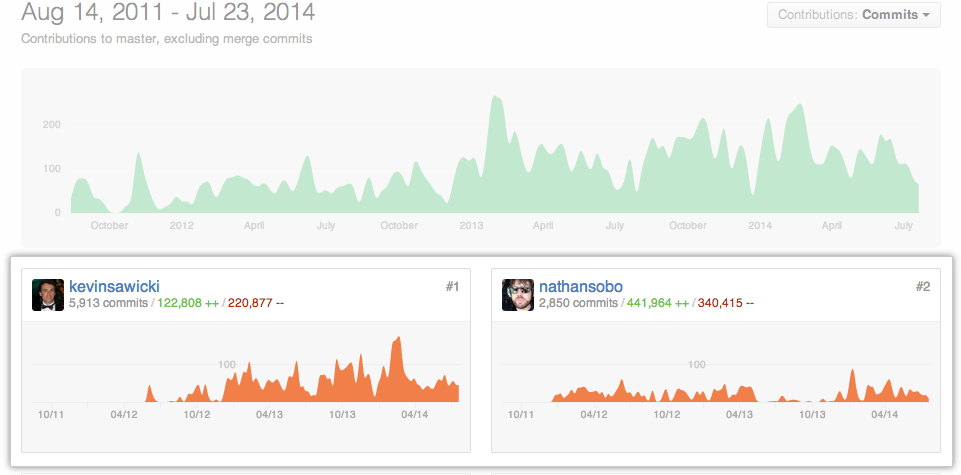
\includegraphics[width=.9\linewidth]{figs/repo_contributors_specific_graph.png}
\end{center}
\end{frame}

\begin{frame}[label={sec:org2a41b7e}]{Estructura de ramas de un repositorio}
\begin{center}
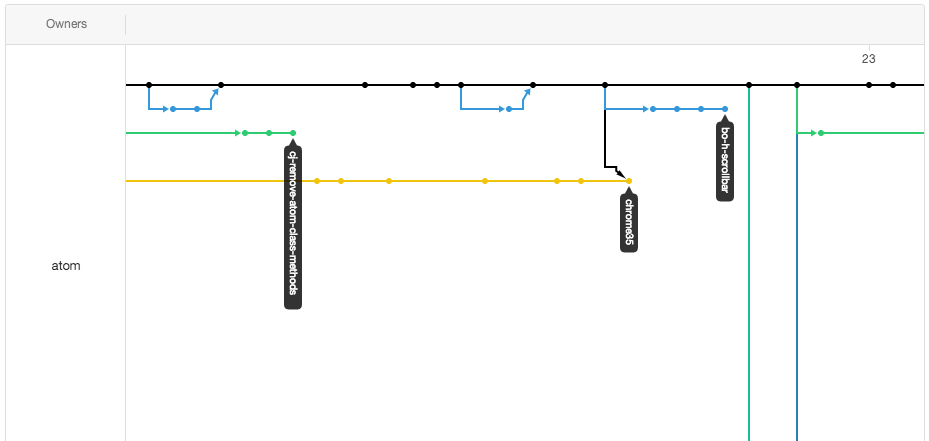
\includegraphics[width=.9\linewidth]{figs/repo_network_graph.png}
\end{center}
\end{frame}

\begin{frame}[label={sec:orgcca1504}]{Cambios en un repositorio}
\begin{center}
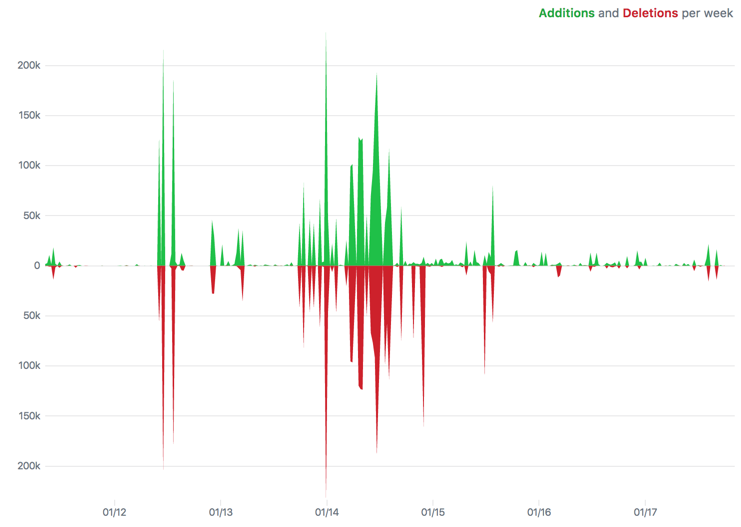
\includegraphics[width=.9\linewidth]{figs/repo_code_frequency_graph_dotcom.png}
\end{center}
\end{frame}

\section{Publicación de páginas web en GitHub}
\label{sec:org6a07271}

\begin{frame}[fragile,label={sec:org082b8c2}]{Página web de usuario u organización}
 \begin{enumerate}
\item Crea un repositorio nuevo con el nombre \texttt{<username>.github.io}\footnote{Siendo \texttt{<username>} tu nombre de usuario en GitHub.}.
\item Sube (\texttt{commit} + \texttt{push}) un fichero \texttt{index.html} a la rama \texttt{master} con código HTML.
\item Con un navegador ve a la dirección \url{https://<username>.github.io}
\end{enumerate}

\lstset{language=HTML,label= ,caption= ,captionpos=b,numbers=none}
\begin{lstlisting}
<!DOCTYPE HTML>
<html>
	<head>
		<title>Hello World</title>
	</head>
	<body>
		Hello World!
	</body>
</html>
\end{lstlisting}
\end{frame}

\begin{frame}[fragile,label={sec:org1ce4ebb}]{Página web de proyecto}
 \begin{block}{Si no sabes HTML}
\begin{itemize}
\item En la página del repositorio:
\end{itemize}

\begin{center}
\boxed{Settings > GitHub\ Pages > Source > master\ branch}

\boxed{Settings > GitHub\ Pages > Theme\ Chooser}
\end{center}

\begin{itemize}
\item Modifica el fichero \texttt{README.md}\footnote{Más información sobre formato Markdown \url{https://guides.github.com/features/mastering-markdown/}.} (\texttt{commit} + \texttt{push}).

\item Con un navegador ve a la dirección \url{https://<username>.github.io/<repository>}
\end{itemize}
\end{block}
\end{frame}

\begin{frame}[fragile,label={sec:orgb0c6533}]{Página web de proyecto}
 \begin{block}{Si sabes HTML}
\begin{itemize}
\item Crea una carpeta \texttt{docs} en la rama \texttt{master} del repositorio.

\item En esta carpeta \texttt{docs} crea/modifica un fichero \texttt{index.html} (\texttt{commit} + \texttt{push}).

\item En la página del repositorio:
\end{itemize}

\begin{center}
\boxed{Settings > GitHub\ Pages > Source > docs\ folder}
\end{center}

\begin{itemize}
\item Con un navegador ve a la dirección \url{https://<username>.github.io/<repository>}
\end{itemize}
\end{block}
\end{frame}
\end{document}